共享数据的并发(同时)访问是一个性能杀手。因为为了避免数据竞争,在给定的时间内只有一个线程可以操作共享数据。可以使用互斥量来完成这个任务,如果有原子操作的话,可以使用原子操作。无论哪种方式,当一个线程递增共享变量时,其他所有线程都必须等待。上一节的测试结果也证实了这一点。

然而,在根据观察和测试采取任何行动前,要理解我们测试了什么,以及可以确定地得出什么结论。

多个线程同时递增一个共享变量根本没有扩展性,甚至比只使用一个线程还要慢,原子共享变量和互斥保护的非原子变量都是如此。这里没有尝试测试对非原子变量的无保护访问,因为这样的操作会导致未定义行为和不正确的结果。对特定于线程(非共享)变量的无保护访问,可以很好地随着线程的数量而扩展,至少在饱和了内存带宽前是这样(这只会发生在写大量数据的时候;对于单个变量来说,这不是问题)。批判性地、不带偏见地分析实验结果是一项重要的技能,有保护的访问共享数据很慢,而无保护的访问非共享数据很快。如果由此得出共享数据会使程序变慢的结论,就需要做出一个假设:\textbf{共享数据}重要,而\textbf{访问保护}不重要。这就引出了在进行性能测量时的另一个问题:比较程序的两个版本时,一次只更改其中一个的内容,然后测试结果。

我们缺少对受保护数据的非共享访问的衡量标准。当然,这里不需要保护单线程的数据访问,但我们试图理解是什么原因使共享数据的访问有如此大开销。是共享或是原子的原因(或由锁保护)?为了确定这一点,需要一次做一个更改,所以保持原子访问并删除数据共享。第一种方法是创建一个原子变量的全局数组,并让每个线程访问自己的数组元素:

\hspace*{\fill} \\ %插入空行
\noindent
\textbf{04\_local\_incr.C}
\begin{lstlisting}[style=styleCXX]
std::atomic<unsigned long> a[1024];
void BM_false_shared(benchmark::State& state) {
	std::atomic<unsigned long>& x = a[state.thread_index];
	for (auto _ : state) {
		benchmark::DoNotOptimize(++x);
	}
}
\end{lstlisting}

谷歌基准测试中的线程索引对于每个线程都是唯一的,数字从0开始,并且是紧凑的(0,1,2…)。另一种简单的方法是在基准函数中声明变量,如下所示:

\hspace*{\fill} \\ %插入空行
\noindent
\textbf{04\_local\_incr.C}
\begin{lstlisting}[style=styleCXX]
void BM_not_shared(benchmark::State& state) {
	std::atomic<unsigned long> x;
	for (auto _ : state) {
		benchmark::DoNotOptimize(++x);
	}
}
\end{lstlisting}

现在,对同一个原子整数进行递增,就像为图5.4收集测试数据时所做的那样,只是现在不再在线程之间共享。这将说明性能变差是共享的原因,还是原子变量的原因。以下是结果:

%\hspace*{\fill} \\ %插入空行
\begin{center}
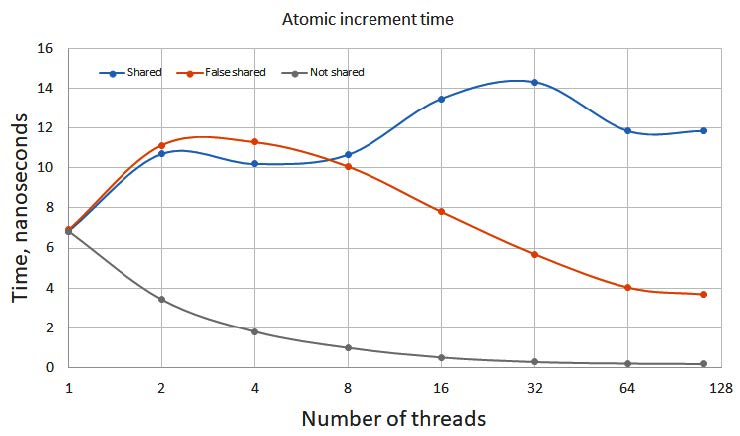
\includegraphics[width=0.9\textwidth]{content/1/chapter5/images/6.jpg}\\
图5.6 - 共享和非共享变量的原子增量时间
\end{center}

图5.4中的的\textbf{Shared}曲线为共享数据的曲线,另外两条曲线为不共享数据的曲线。线程上都有一个局部变量的基准测试标记为\textbf{Not shared}。在两个线程上的计算时间比在一个线程上的计算时间少一半,在四个线程上的计算时间又减少了一半,以此类推。请记住,这是一个增量操作的平均时间,总共做了100万次增量计算,测试它所花费的总时间,然后除以100万。由于递增的变量不是在线程之间共享的,所以期望两个线程的运行速度是一个线程的两倍,所以\textbf{Not shared}的结果与期望相符。另一个基准测试中,使用原子变量数组,但每个线程使用自己的数组元素,也没有共享数据。然而,其执行就像数据在线程之间共享一样,至少对于少量的线程是这样,所以称它为\textbf{伪共享}:没有什么是真正共享的,但程序的行为就像是共享的一样。

这个结果表明,数据共享成本高的原因比之前假设的要复杂。在伪共享的情况下,只有一个线程在操作每个数组元素,所以不需要等待任何其他线程完成其增量操作。然而,线程显然在彼此等待。为了理解这种异常现象,必须对缓存的工作方式进行更多的了解。

在多核或多处理器系统中,数据在处理器和内存之间移动的方式如图5.7所示。

%\hspace*{\fill} \\ %插入空行
\begin{center}
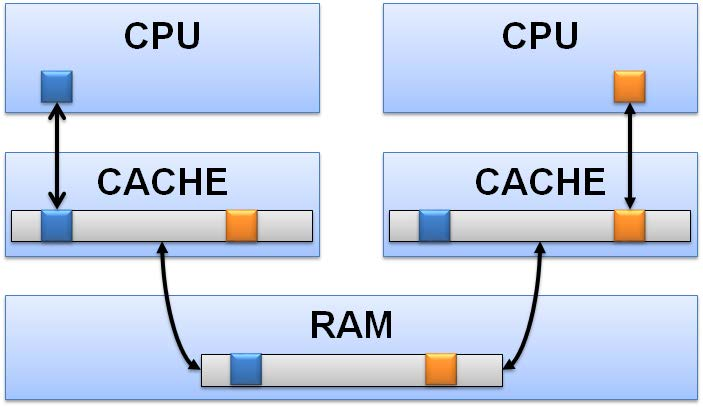
\includegraphics[width=0.6\textwidth]{content/1/chapter5/images/7.jpg}\\
图5.7 - 多核系统中CPU和内存之间的数据传输
\end{center}

处理器以字节或整数的形式处理数据,这取决于变量的类型。在我们的例子中,一个\texttt{unsigned long}类型变量具有8字节。原子增量读取指定地址处的单个字,对其加1,然后写回。但是从哪里读呢?CPU只能直接访问L1缓存,因此只能从那里获取数据。数据如何从主存储器进入高速缓存?数据是通过内存总线复制的,而内存总线要宽得多。可以从内存复制到高速缓存并返回的最小数据量称为\textbf{缓存行}。在所有x86 CPU上,一条缓存行的大小为64字节。当CPU需要为一个原子事务锁定内存位置时,比如一个原子增量,CPU可能在写一个数据,并锁定整个缓存行:如果两个CPU可以在同一时间将同一缓存行写入内存,那么其中一个必然会覆盖另一个。注意,为了简单起见,在图5.7中只显示了一个级别的缓存层次结构,但这没有区别。数据会以缓存行长的形式经过所有级别的缓存。

现在可以解释我们观察到的伪共享。即使相邻的数组元素在线程之间并没有真正共享,但确实占用了相同的缓存行。当CPU请求独占访问一个数组元素时,会锁定整个缓存行,阻止其他CPU访问其中的任何数据。这也解释了为什么图5.7中的伪共享在8个线程时看起来和真正的数据共享是一样的,但是在更多的线程时变得更快:写入的是8个字节的数据,所以它们中的8个可以放进同一个缓存行中。如果只有8个线程(或更少),那么在任何给定的时间,只有一个线程可以增加它的值,这与真正的共享一样。但是如果超过8个线程,数组至少占用两条缓存行,并且可以被两个独立的CPU锁住。所以,若有16个线程,那么就有两个线程可以向前移动,数组的一半对应一个线程。

另一方面,真正的非共享基准测试在每个线程的堆栈上分配原子变量。是完全独立的内存分配,由许多缓存行隔开。由于没有内存交互,这些线程可以完全独立地运行。

分析表明,访问共享数据的高成本的真正原因是,必须维护对缓存行的独占访问,并确保所有CPU的缓存中有一致的数据。当一个CPU获得了独占访问权,并且更新了缓存行上的1位后,所有其他CPU的缓存行副本就过期了。在其他CPU访问同一缓存行的数据之前,必须从主存中获取更新后的内容,这将花费较长的时间。

两个线程是否访问相同的内存位置并不重要,重要的是它们会竞争访问相同的缓存行。独占的缓存行访问是共享变量高成本的根源。

有人可能想知道,锁昂贵的原因是否也存在于包含的共享数据中(所有锁都必须具有一定数量的共享数据,这是一个线程可以让另一个线程知道锁占用的唯一方法)。即使是在一个线程上,互斥锁也比单个原子访问要昂贵得多,如图5.4和5.5中看到的那样。锁定互斥对象比仅仅修改一个原子变量需要更多的工作。但是,当有多个线程时,为什么这项工作要花费更多的时间呢?是因为数据是共享的,需要独占的访问缓存行吗?我们把这个问题留给读者作为一个练习,通过自己的方法确认是否真的是这样。这个问题的关键是设置锁的伪共享。一个锁数组,每个线程操作自己的锁,竞争相同的缓存行(当然,这种每个线程的锁实际上并不能保护并发访问,但我们想要的是锁定和解锁所花费的时间)。标准C++的互斥量\texttt{std::mutex}通常相当大,根据操作系统的不同,在40到80字节之间,可能不能在同一个缓存行中放入两个互斥量。所以必须使用较小的锁来进行这个实验,例如:自旋锁或futex(fast userspace mutex)。

现在明白了为什么并发访问共享数据的代价如此之高。这里需要注意两点:首先,创建非共享数据时,要避免错误的数据共享。无意间的错误共享会在程序出现吗?这一章已经有了个简单的例子:对多个数进行同时累加求和。我们的方法都非常慢(比单线程程序慢,或者和单线程性能相当),同时也清楚了访问共享数据的开销很高。那么,有什么方法能降低这个开销呢?当然,不是访问共享数据!至少是不经常访问它。对于我们来说,不需要在想要进行累加时,就访问共享内存。我们可以在本地、线程上进行累加,并在最后一次性将它们添加到共享的累加值中:

\hspace*{\fill} \\ %插入空行
\noindent
\textbf{04\_local\_incr.C}
\begin{lstlisting}[style=styleCXX]
// Global (shared) results
std::atomic<unsigned long> sum;
unsigned long local_sum[…];
// Per-thread work is done here
unsigned long& x = local_sum[thread_index];
for (size_t i = 0; i < N; ++i) ++x;
sum += x;
\end{lstlisting}

我们有一个全局结果\texttt{sum},它在所有线程之间共享,并且必须是原子的(或者由锁保护)。但是在所有的工作完成后,每个线程只访问这个变量一次。每个线程使用另一个变量来保存部分和,只保存在该线程上添加的值(在我们的简单示例中,增量为1,但无论添加的值是什么,性能都是相同的)。我们可以创建一个大数组来存储每个线程的部分和,并给每个线程一个单独的数组来对元素进行处理。在这个简单的例子中,可以只使用一个局部变量,但是在实际的程序中,部分结果通常需要在工作线程完成之后保存,而这些结果的最终处理可能是通过其他线程完成的。为了模拟这种实现,我们使用每个线程的数组。注意,这些数组中只是普通的整数:不会并发访问。在此过程中,我们落入了错误共享的陷阱:数组的相邻元素(通常)位于同一高速缓存行上,因此不能并发访问。这反映在程序的性能上:

%\hspace*{\fill} \\ %插入空行
\begin{center}
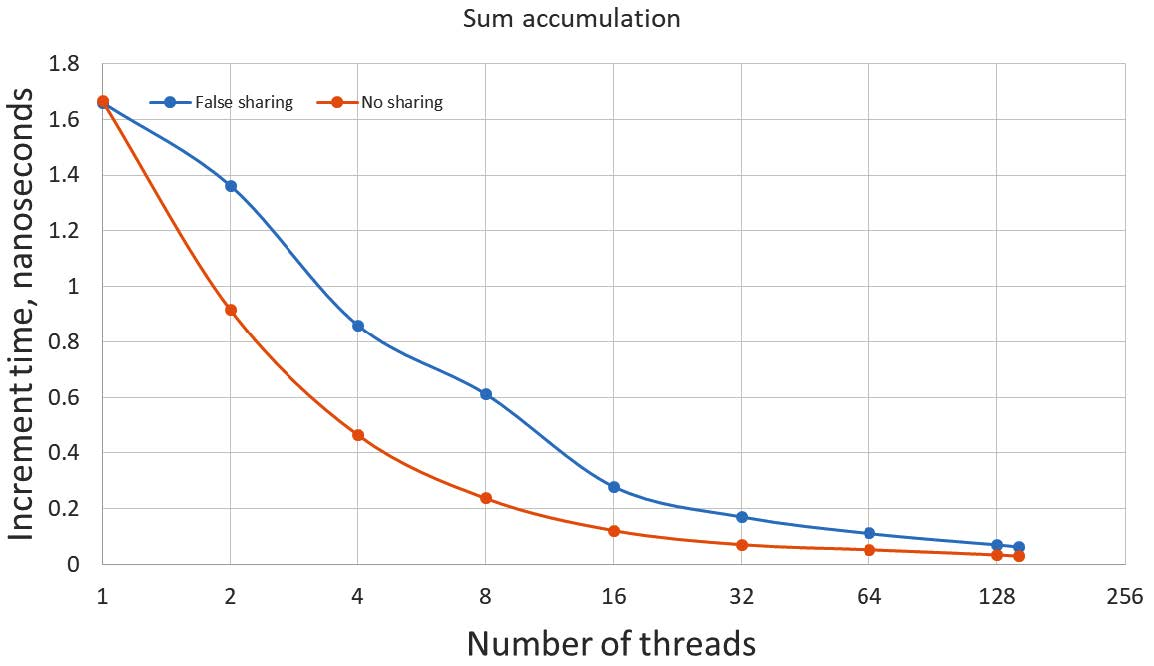
\includegraphics[width=0.9\textwidth]{content/1/chapter5/images/8.jpg}\\
图5.8 - 有与没有伪共享的累加计算
\end{center}

可以在图5.8中看到,程序的扩展性非常差,需要开非常多的线程才会好。另一方面,如果通过确保每个线程的部分和之间,至少有64字节(或者在我们的例子中仅使用局部变量)来消除伪共享,那么就可以完美地扩展。当使用更多的线程时,两个程序都会变得更快,但不受伪共享影响的实现性能,可以是单线程的(大约)两倍。

第二点将在后面的章节中变得更加重要。由于并发访问共享变量相对来说非常昂贵,因此使用较少共享变量的算法或实现通常会执行得更快。

目前,这种说法可能令人困惑。问题的本质是,有一些必须共享的数据。可以像刚才那样进行优化,并消除对该数据的不必要访问。完成后,剩下的就是需要访问的数据,以产生所需的结果。那么,共享变量怎么可能更多或更少呢?要理解这一点,必须了解,好的并发代码比保护对所有共享数据的访问更重要。






































